\documentclass[10pt,a4paper]{article}
\usepackage[top=15mm,bottom=16mm,left=18mm,right=18mm,headheight=13pt,headsep=5mm]{geometry}
\usepackage[T1]{fontenc}
\usepackage{lmodern}
\usepackage{amsmath,amssymb,graphicx,booktabs,tabularx,array,xcolor}
\usepackage{fancyhdr,titlesec,caption,listings,microtype}
\usepackage{eso-pic}
\usepackage[hidelinks]{hyperref}
\hypersetup{colorlinks=true,allcolors=black,pdftitle={EN3160 Assignment 02: Fitting and Alignment},pdfauthor={Dilhan W.A.}}
\pagestyle{fancy}
\fancyhf{}
\fancyhead[L]{\small EN3160 -- Assignment 02}
\fancyhead[R]{\small Index No.: 230145E}
\fancyfoot[C]{\small\thepage}
\renewcommand{\headrulewidth}{0.4pt}
\renewcommand{\footrulewidth}{0pt}
\setlength{\parindent}{0pt}
\setlength{\parskip}{3.5pt}
\setlength{\tabcolsep}{5pt}
\renewcommand{\arraystretch}{1.12}
\titleformat{\section}{\large\bfseries}{\thesection.}{0.55em}{}
\titlespacing*{\section}{0pt}{7pt}{4pt}
\captionsetup{font=footnotesize,labelfont=bf,skip=3pt,hypcap=false}
\lstset{language=Python,basicstyle=\ttfamily\scriptsize,keywordstyle=\bfseries,
 commentstyle=\itshape,stringstyle=\ttfamily,frame=tb,rulecolor=\color{black},
 aboveskip=5pt,belowskip=5pt,showstringspaces=false,breaklines=true,
 xleftmargin=0pt,framexleftmargin=2pt,framesep=3pt}
\color{black}
% Generated from measured experiment outputs; do not edit by hand.
\newcommand{\BlobCount}{53}
\newcommand{\BlobRows}{%
1 & 282 & 338 & 7.106 & 10.050 & 0.351 \\
2 & 106 & 255 & 5.801 & 8.204 & 0.365 \\
3 & 179 & 327 & 5.801 & 8.204 & 0.346 \\
4 & 178 & 261 & 5.422 & 7.668 & 0.353 \\
5 & 274 & 258 & 4.736 & 6.698 & 0.347 \\
}
\newcommand{\FitRows}{%
Line & $a=0.7210,\ b=0.6930,\ d=1.5724$ & 54 & 0.6706 \\
Circle & $c_x=1.9494,\ c_y=2.9879,\ r=9.8919$ & 46 & 0.5925 \\
}
\newcommand{\PcbRows}{%
AAAA1 & 38 & 15 & 0.944 & 89.0\% & 29.31 \\
ADAD1 & 252 & 187 & 0.439 & 98.1\% & 30.62 \\
AECC2 & 3314 & 3068 & 0.210 & 98.3\% & 3.52 \\
AECC3 & 3978 & 3664 & 0.167 & 98.8\% & 3.29 \\
AECC4 & 3171 & 2913 & 0.231 & 98.4\% & 4.07 \\
}
\newcommand{\CornerRows}{%
Studio & (215,405), (953,508), (953,556), (215,461) & 0.82 \\
Garden & (454,683), (782,683), (786,800), (450,800) & 0.78 \\
}

\newcommand{\figcaption}[1]{\captionof{figure}{#1}}
\newcommand{\smallnote}[1]{{\footnotesize #1\par}}

\begin{document}
% Cover coordinates and type sizes reproduce the supplied reference layout.
% Coordinates are PDF points measured from the top of the A4 page.
\thispagestyle{empty}
\newcommand{\coverline}[4]{\put(297.6378,-#1){\makebox[0pt][c]{\fontsize{#2bp}{#2bp}\selectfont #3#4}}}
\AddToShipoutPictureFG*{\setlength{\unitlength}{1bp}\AtPageUpperLeft{%
\put(244.260,-230.376){
\includegraphics[width=106.757bp,height=113.386bp]{figures/uom_logo.png}}
\coverline{282.0}{11.9552}{\bfseries}{Department of Electronic \& Telecommunication Engineering}
\coverline{314.1}{11.9552}{\bfseries}{University of Moratuwa, Sri Lanka}
\coverline{381.0}{14.3462}{\bfseries}{EN3160 - Assignment 02}
\coverline{435.2}{17.2154}{\bfseries}{Fitting and Alignment}
\coverline{460.1}{17.2154}{\bfseries}{in Computer Vision}
\coverline{510.1}{11.9552}{}{Submitted by}
\coverline{542.2}{11.9552}{\bfseries}{230145E\quad Dilhan W.A.}
\coverline{588.5}{11.9552}{}{B.Sc. Engineering - Semester 05}
\coverline{620.6}{11.9552}{}{EN3160}
\coverline{661.2}{11.9552}{}{October 19, 2026}
}}
\null\newpage

\section{Sunflower detection using scale-space extrema}
\smallnote{\textbf{Repository:} \url{https://github.com/ahesh-dilhan/en3160-assignment-02}}
The supplied image is read with \texttt{cv.IMREAD\_REDUCED\_COLOR\_4}, giving
$360\times360$ pixels. The detector targets dark central disks rather than
irregular petal outlines. For darkness $D=1-I_{\mathrm{gray}}/255$, the response is
$L(x,y,\sigma)=-\sigma^2\nabla^2(G_\sigma*D)$; positive maxima identify dark blobs
in the original image. The ideal-disk radius estimate is $r=\sqrt{2}\sigma$.

\begin{lstlisting}
L = np.stack([-s*s*gaussian_laplace(D, s) for s in sigmas])
peaks = (L == maximum_filter(L, size=(3, 3, 3))) & (L >= 0.12)
\end{lstlisting}
\textbf{Parameters.} There are 36 geometrically spaced scales,
$\sigma\in[1.5,16]$ pixels; end-scale maxima are excluded. The threshold is 0.12
and allowed disk overlap is 35\% of the smaller area. A yellow-petal prior requires
50\% yellow support in the annulus $[r,2.2r]$, with angular coverage. A Hessian
curvature ratio of at least 0.5 rejects elongated gaps. No Hough-circle detector is used.

\begin{center}
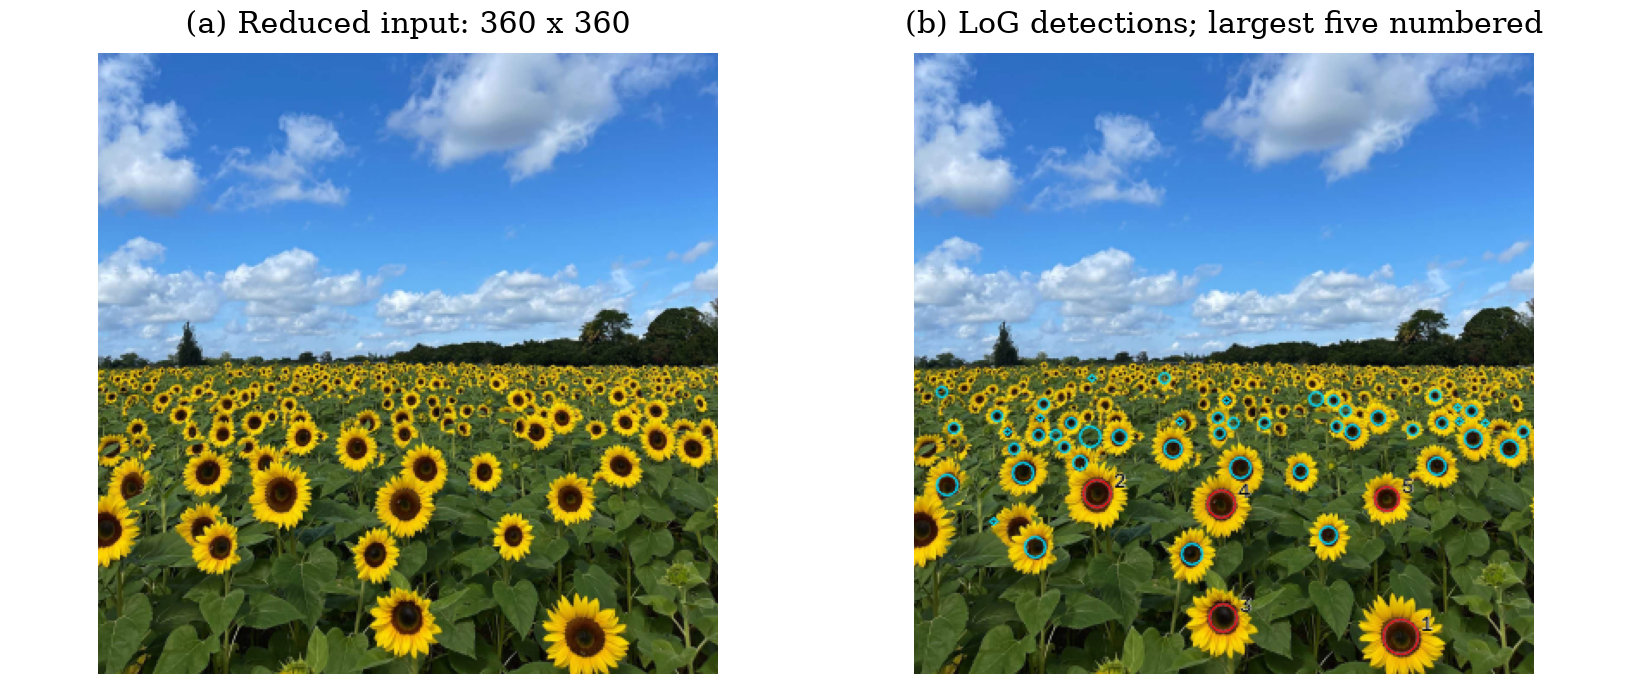
\includegraphics[width=0.91\linewidth]{figures/sunflowers.png}
\figcaption{Original-colour input and \BlobCount{} detected candidates.
The five largest central disks are numbered in the right panel.}
\end{center}
\vspace{-4pt}
\begin{center}\small
\begin{tabular}{rrrrrr}
\toprule Rank & $x$ & $y$ & $\sigma$ (px) & $r$ (px) & Response \\ \midrule
\BlobRows
\bottomrule
\end{tabular}\end{center}
\textbf{Interpretation.} The largest disk is centred at $(282,338)$ with
$r=10.05$ pixels. Coordinates use the top-left origin of the reduced image;
multiply positions and radii by four for original-image units. Colour and
symmetry checks suppress foliage responses but miss distant, tilted or occluded
flowers. These are candidate detections, not a verified flower count; the
estimated radii describe central disks, not complete blossoms.

\newpage
\section{Custom RANSAC fitting: line followed by circle}
\textbf{Data and hypotheses.} Listing 1 is reproduced with data seed 0: 50 circle
points with centre $(2,3)$, radius 10 and radial-noise standard deviation 0.625,
plus 50 points from $y=-x+2$ with vertical-noise standard deviation 1. Both RANSAC
loops are coded directly. A line hypothesis uses two distinct points; a circle
uses three non-collinear points. Degenerate samples are rejected. Each model
uses 2,000 trials; the sequence starts with RNG seed 100.

\textbf{Residuals and constraints.} The line is $ax+by=d$ with $a^2+b^2=1$ and
$d\geq0$. Its error is perpendicular distance, not vertical distance. The circle
uses radial error. Both thresholds are 1.5, approximately 2.12 normal-noise
standard deviations for the true line and 2.4 for the circle:
\[
 e_\ell(\mathbf p)=|ap_x+bp_y-d|,\qquad
 e_c(\mathbf p)=\bigl|\|\mathbf p-\mathbf c\|_2-r\bigr|.
\]
The first line needs at least 35 inliers. Its best consensus is removed, after
which the circle needs at least 25. Total least squares refines the line;
L-BFGS-B minimizes mean squared radial error with $r>0$. Consensus membership is
updated after refinement. Winning minimal samples and their unrefined models
are retained separately.

\begin{lstlisting}
line = ransac(X, "line", rng, threshold=1.5, minimum_consensus=35)
remaining = np.flatnonzero(~line.inliers)
circle = ransac(X[remaining], "circle", rng,
                threshold=1.5, minimum_consensus=25)
\end{lstlisting}
\begin{center}
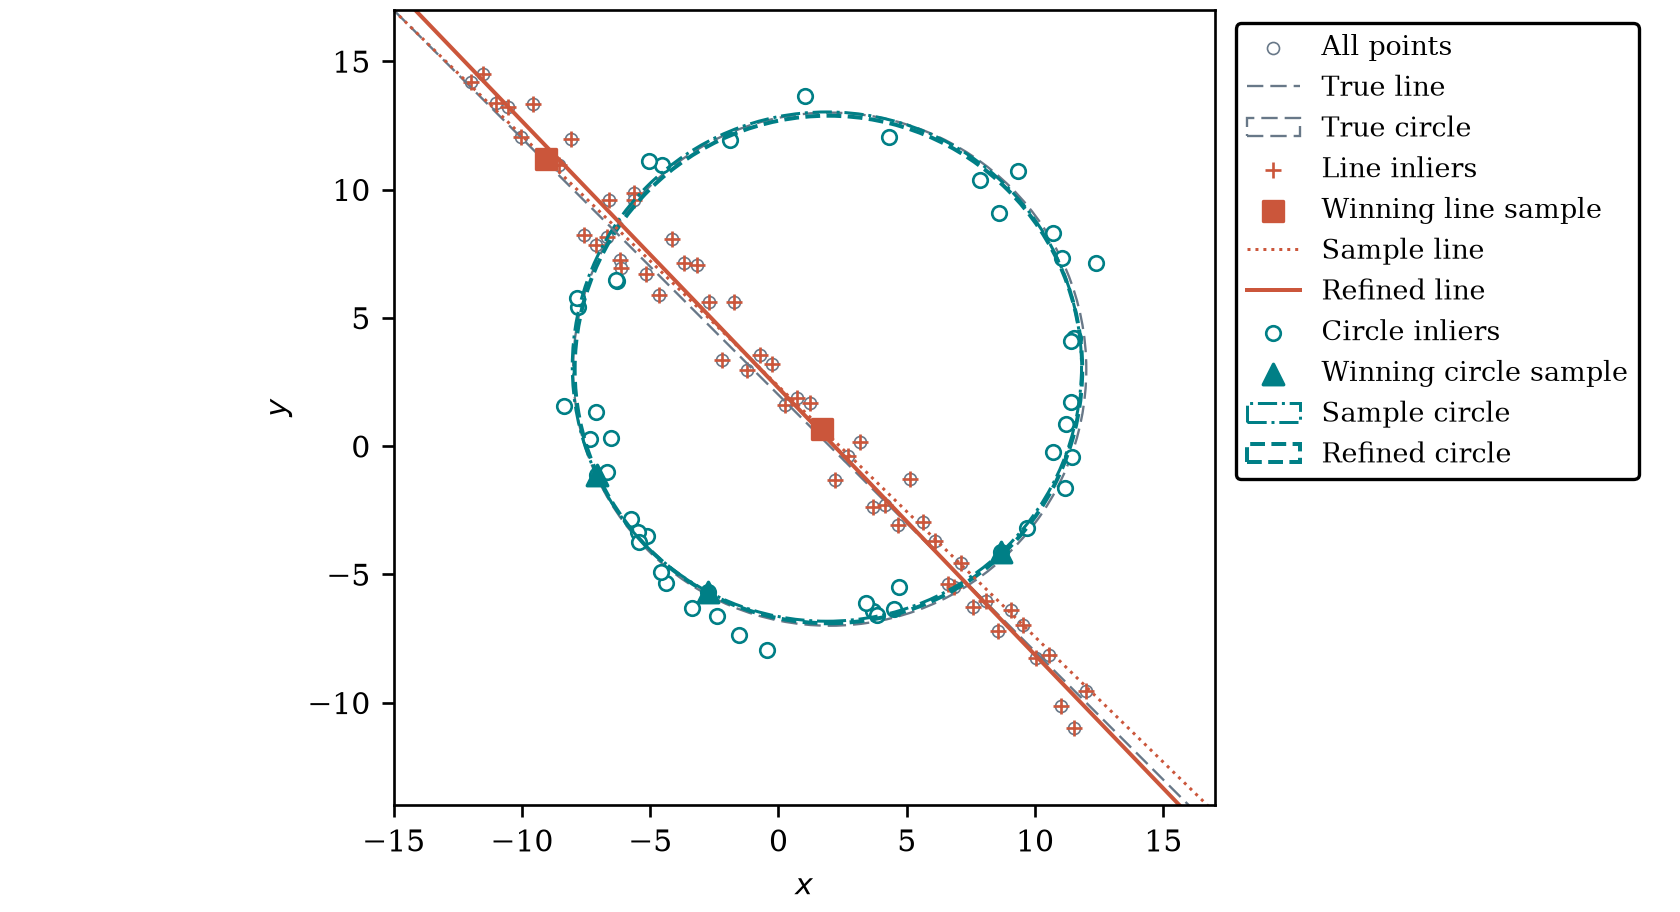
\includegraphics[width=\linewidth]{figures/ransac.png}
\figcaption{All points, winning line and circle samples, sample hypotheses,
refined models and their consensus sets. Markers and line styles distinguish
models; all labels and text remain black.}
\end{center}
\vspace{-4pt}
\begin{center}\small
\begin{tabular}{l l r r}
\toprule Model & Refined parameters & Inliers & Inlier RMSE \\ \midrule
\FitRows
\bottomrule
\end{tabular}\end{center}
\textbf{Iteration budget.} For confidence $p=0.99$ and a hypothetical inlier
fraction $w=0.5$, $N=\lceil\log(1-p)/\log(1-w^s)\rceil$ gives 17 trials for
$s=2$ and 35 for $s=3$. The larger fixed budget accommodates contamination and
lower inlier fractions after consensus removal; it does not guarantee success.

\textbf{Circle first.} Seed 0 also succeeds in this order: centre
$(1.943,3.008)$ and radius 9.930. Across data seeds 0--19, circle recovery occurs
in 20/20 line-first runs and 19/20 circle-first runs, using centre and radius
errors below 2 as the declared criterion. A very large circle can approximate a
line and claim its points, so circle-first is vulnerable but does not always
fail. Line-first also removes some genuine circle points near intersections,
explaining its consensus of 54. Geometric refinement is local, not proof of a
global optimum.

\newpage
\section{Planar homography and image compositing}
\textbf{Choice of image pairs.} Two architectural photographs are paired with
original graphic overlays: a fictional open-studio banner on a flat band of a
modern facade, and a community-garden notice on a garage door. The first gives
an oblique placement and the second a nearly frontal comparison. These notices
do not describe actual events or imply endorsement by property owners.

Four manually selected destination corners are ordered top-left, top-right,
bottom-right, bottom-left. They were selected from visual inspection; actual
mouse clicks have not been recorded. The supplied \texttt{select\_corners.py}
script supports repeatable four-click selection. The saved coordinates and
blend weights are listed below.

\begin{center}
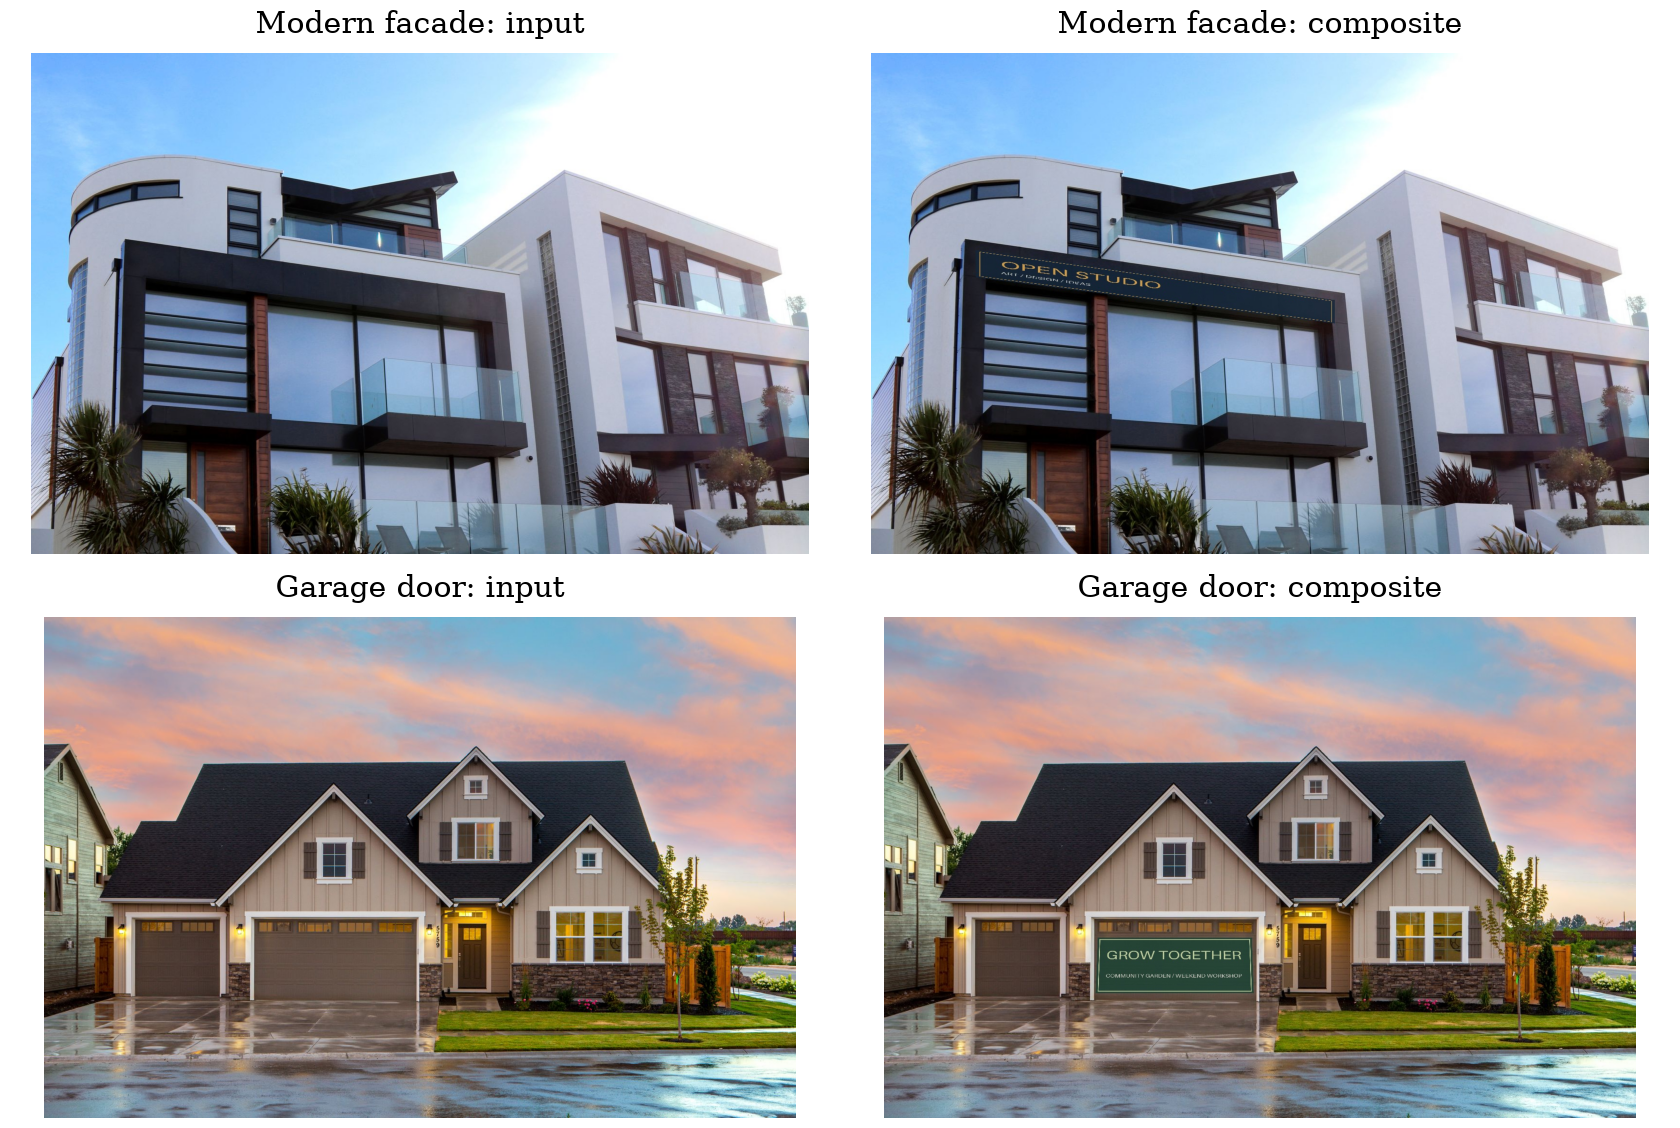
\includegraphics[width=\linewidth]{figures/composites.png}
\figcaption{Two chosen architectural image pairs, retaining their original colours.
Each row compares the input photograph with its composited result.}
\end{center}
\vspace{-4pt}
\textbf{Mapping and blending.} The four source corners and four destination
corners define $H$, mapping overlay coordinates to background coordinates:
$\mathbf x'\sim H\mathbf x$. The graphic and an all-one coverage mask are warped
with identical bilinear interpolation. Using premultiplied warped colour $W$
and coverage $M$, the result is $C=B(1-\alpha M)+\alpha W$. Black graphic pixels
remain valid content; coverage is independent of pixel brightness.

\begin{lstlisting}
H = cv.getPerspectiveTransform(source_corners, destination_corners)
W = cv.warpPerspective(overlay.astype(np.float32), H, size)
M = cv.warpPerspective(np.ones((h, w), np.float32), H, size)
result = background*(1-alpha*M[..., None]) + alpha*W
\end{lstlisting}
\begin{center}\footnotesize
\begin{tabular}{l l r}
\toprule Pair & Destination corners (image pixels) & $\alpha$ \\ \midrule
\CornerRows
\bottomrule
\end{tabular}\end{center}
\textbf{Assessment.} Both homographies reproduce their selected corners to
within 0.001 pixels. This tests point correspondence, not real-world accuracy:
the same four pairs define the transform exactly and are not independent
validation. Alpha blending retains some surface texture but does not model
physical illumination, shadows, reflections or occlusion. The facade band is
more perspective-distorted than the garage placement.

\smallnote{\textbf{Image credits.} Expect Best, \emph{Modern Building Against Sky},
Pexels photo 323780; Binyamin Mellish, \emph{Brown and Gray Painted House in Front
of Road}, Pexels photo 1396122. Both were downloaded at width 1600 and modified
with original graphics. Source pages:
\href{https://www.pexels.com/photo/modern-building-against-sky-323780/}{pexels.com, photo 323780};
\href{https://www.pexels.com/photo/brown-and-gray-painted-house-in-front-of-road-1396122/}{pexels.com, photo 1396122}.
License: \url{https://www.pexels.com/license/}. Full attribution is retained in the repository.}

\newpage
\section{SIFT-based PCB registration and differences}
\textbf{Registration.} The template is \texttt{AECC1.jpg}. SIFT extracts up to
8,000 features per image at maximum side 1600. \texttt{BFMatcher} uses L2
two-neighbour matching with a 0.72 ratio test. RANSAC estimates the target-to-template
homography with a 3-pixel threshold at feature scale, confidence 0.999 and up to
10,000 trials. The mapping is converted to original-image coordinates before
warping all five targets.

\begin{minipage}[t]{0.48\linewidth}\vspace{0pt}
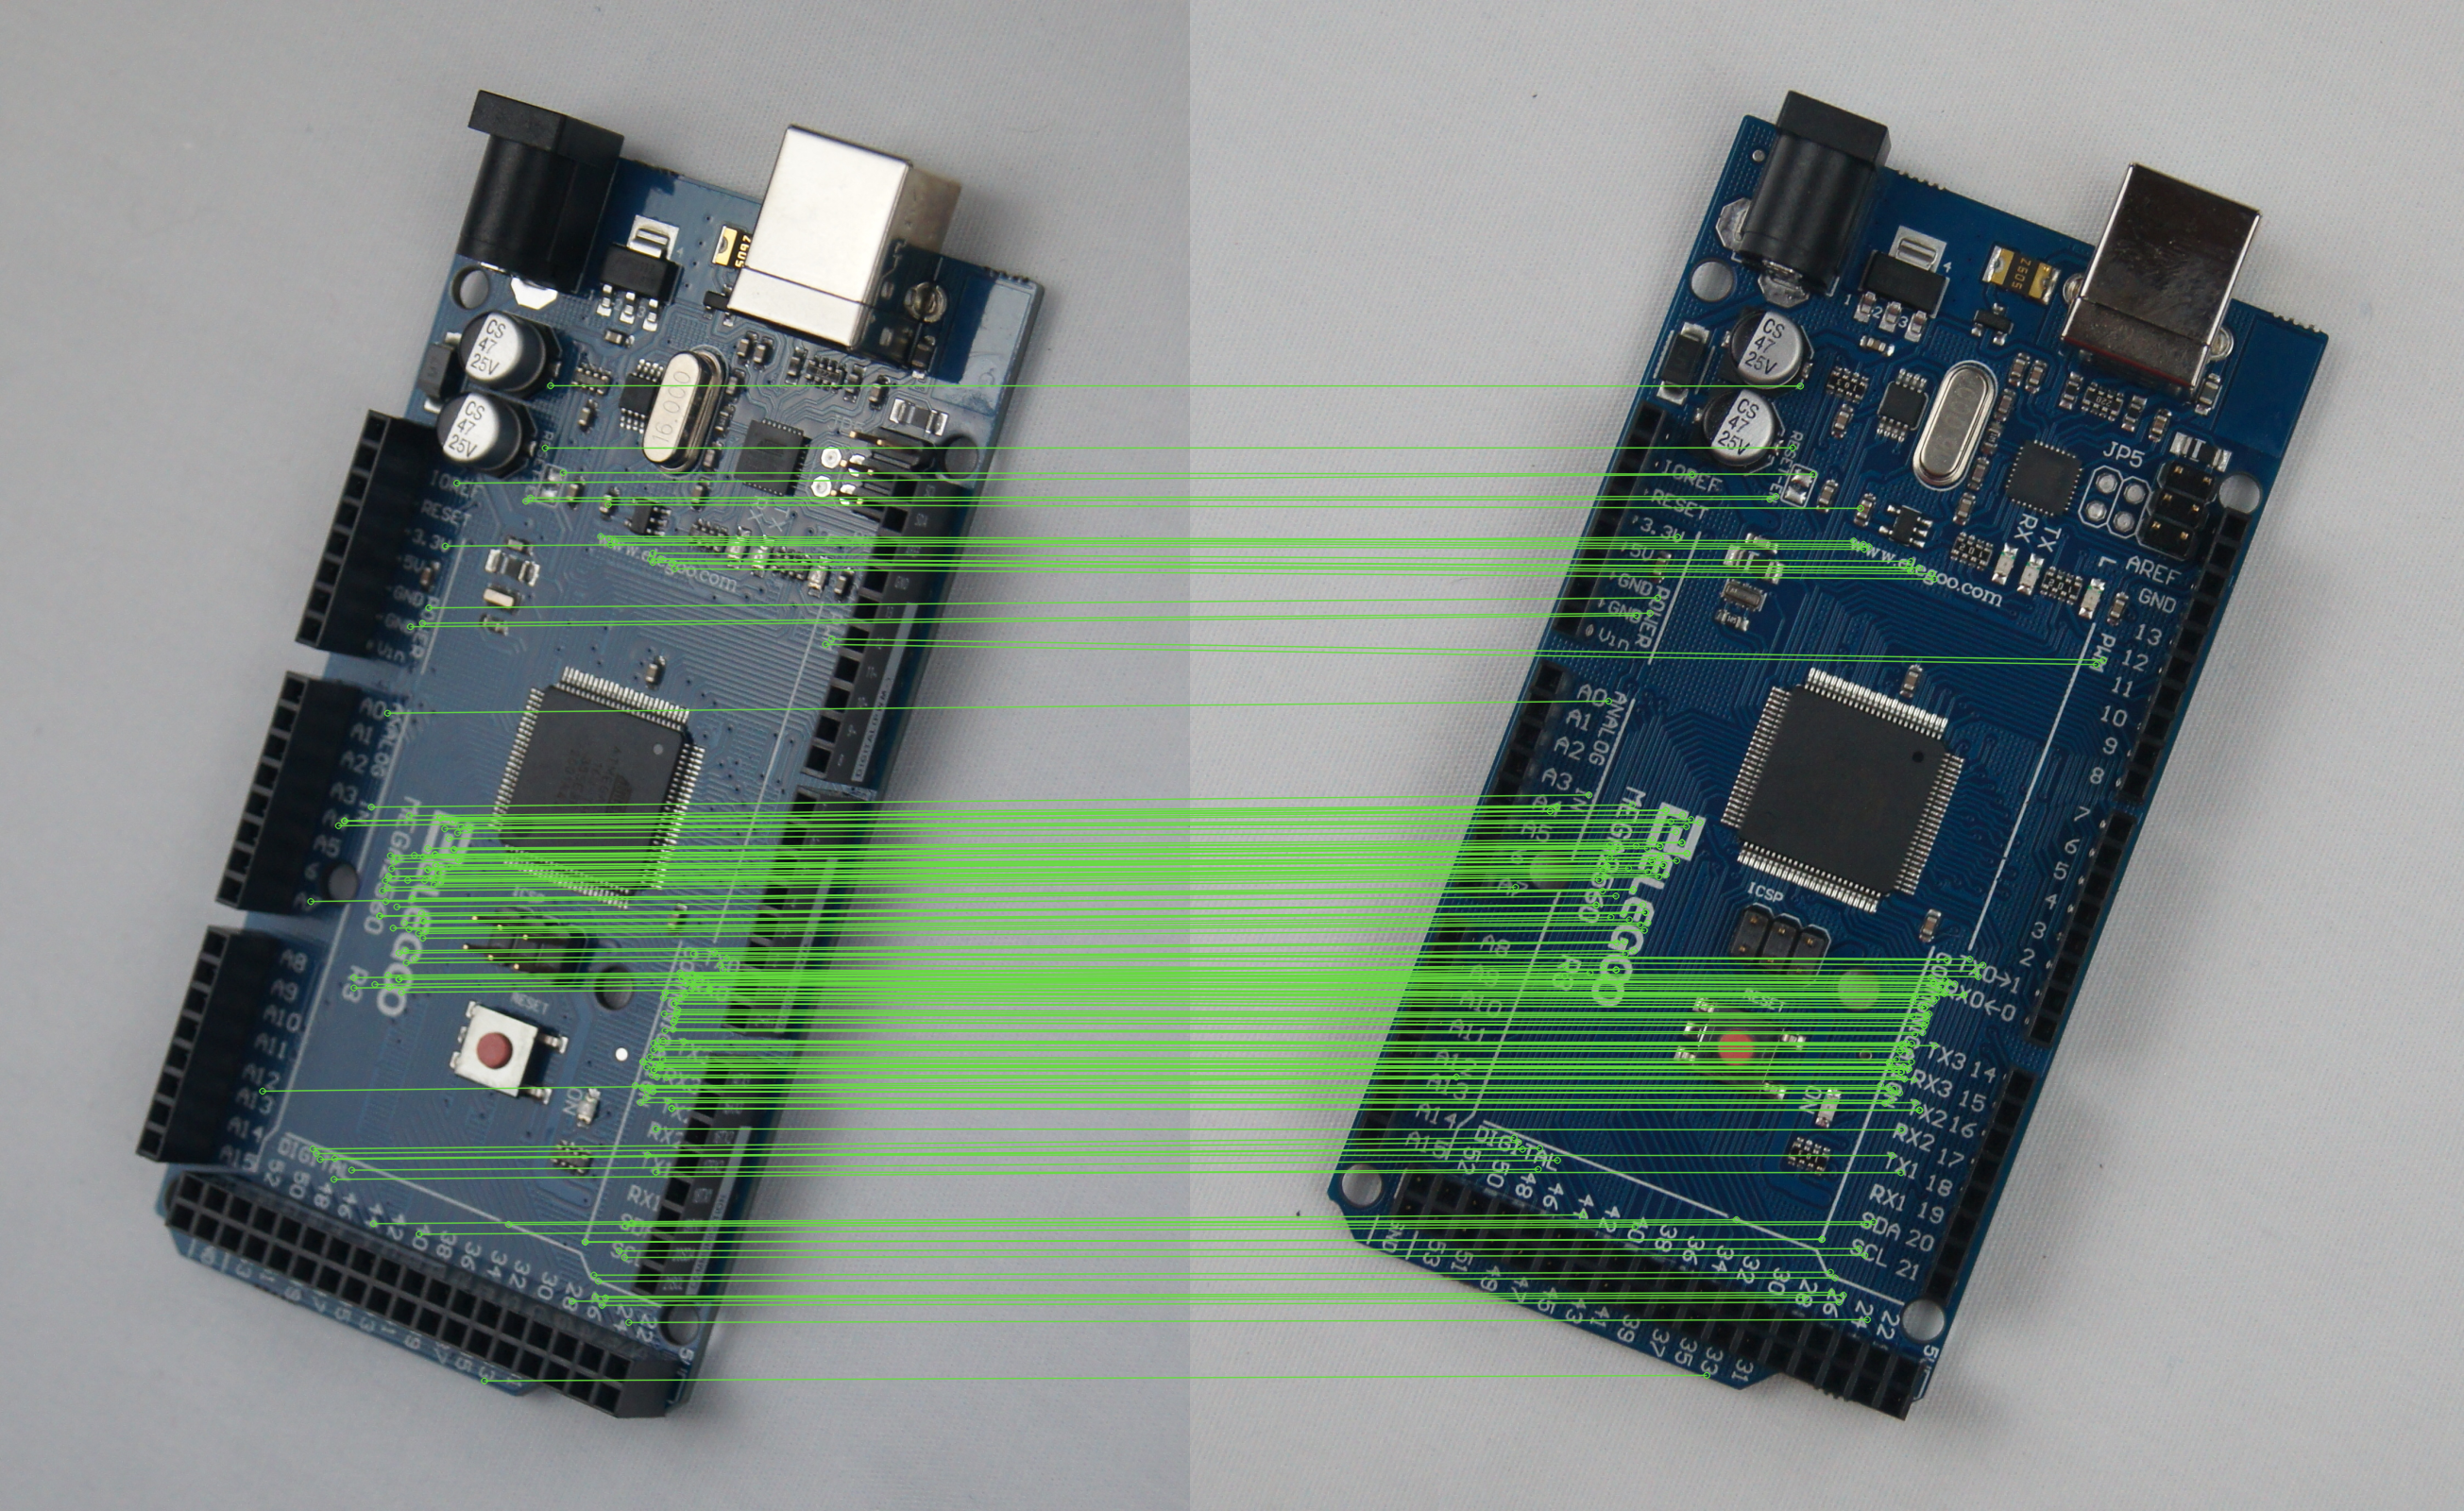
\includegraphics[width=\linewidth]{figures/pcb_matches.png}
\captionof{figure}{ADAD1 to AECC1: green lines show accepted RANSAC matches.}
\end{minipage}\hfill
\begin{minipage}[t]{0.49\linewidth}\vspace{0pt}
\small
\textbf{Registration confidence.} At least eight geometric inliers are required.
AAAA1 has only 15, with an inlier hull spanning 10.1\% of the full template image,
so its large viewpoint change makes it less reliable than AECC2--4. Full-size
match visualizations and alignment overlays are saved in the experiment output
folders.

\textbf{Valid overlap.} An all-one image is warped with the same interpolation.
Partly padded pixels and a one-pixel boundary margin are excluded. This prevents
black warp borders from inflating the difference statistics.
\end{minipage}

\begin{center}
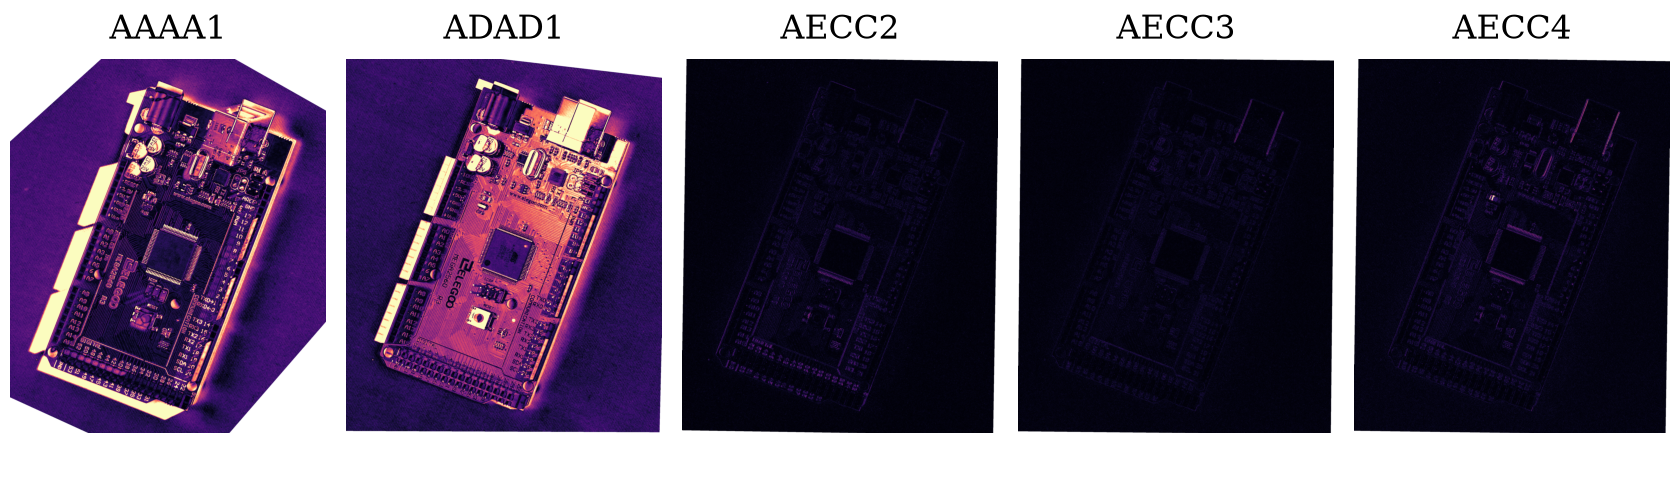
\includegraphics[width=\linewidth]{figures/pcb_differences.png}
\figcaption{Mean absolute RGB differences, displayed with the original magma colour map
over a common 0--100 range: dark is zero and pale yellow is 100 or above. Blank white margins outside
the warped footprint are invalid overlap. Numerical metrics use the full raw values.}
\end{center}
\vspace{-4pt}
\begin{center}\small
\begin{tabular}{l r r r r r}
\toprule Target & Matches & Inliers & Median error$^*$ & Overlap & Raw MAE \\ \midrule
\PcbRows
\bottomrule
\end{tabular}\end{center}
\smallnote{$^*$Median inlier reprojection error, in feature-image pixels.
MAE averages valid RGB-channel differences over the entire overlap, including
background. It is not a board-only defect score. No exposure normalization is applied.}

\begin{lstlisting}
H_full = np.linalg.inv(template_scale) @ H_small @ source_scale
aligned = cv.warpPerspective(target, H_full, template_size)
difference = cv.absdiff(aligned, template)
difference[~valid] = 0
\end{lstlisting}
\textbf{Why raised components differ.} The USB Type B port, capacitors and reset
button lie above the PCB plane. Viewpoint changes cause parallax and occlusion
that one planar homography cannot remove. Specular reflections, shadows,
exposure, residual misalignment and possible component differences also
contribute. AAAA1 and ADAD1 have much larger raw MAE than AECC2--4, consistent
with their stronger viewpoint and appearance changes. Bright residuals alone
do not establish a manufacturing defect.

\smallnote{\textbf{Reproducibility and references.} Ten geometry tests pass,
including unit-normal fitting, robust homography recovery, black-overlay
preservation and valid-overlap masking. Assignment: R. Rodrigo, \emph{EN3160
Assignment 2 on Fitting and Alignment}, 9 October 2026. Optimization background:
S. Boyd and L. Vandenberghe, \emph{Convex Optimization}, \S1.1,
\href{https://web.stanford.edu/~boyd/cvxbook/}{Stanford};
\href{https://docs.scipy.org/doc/scipy/reference/generated/scipy.optimize.minimize.html}{SciPy minimize documentation}.
Code, parameters and genuine commit history:
\url{https://github.com/ahesh-dilhan/en3160-assignment-02}.}
\end{document}
